\section{3D Data Representation}
Modellazione manuale utilizzando software dedicati
Simulazioni
Tecniche di acquisizione attive o passive (scansione laser,
fotogrammetria).
I progressi nelle tecniche di acquisizione hanno finalmente superato il 'bottleneck della modellazione': la creazione di modelli digitali 3D è diventata più semplice e meno costosa.
\subsection{Gemoetry Processing}
La disciplina riguardante modelli matematici per rappresentare dati geometrici e gli algoritmi per analizzarli e manipolarli.
\begin{figure}[H]
    \centering
    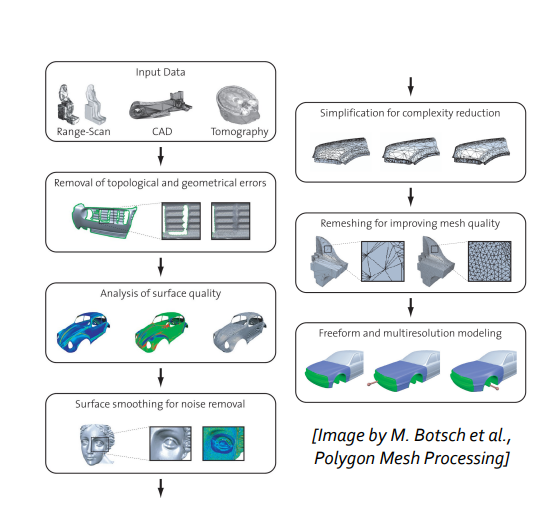
\includegraphics[width=0.5\textwidth]{images/3Drend.png} 
    \caption{Gemoetry Processing}
    \label{fig:immagine}
\end{figure}
\subsubsection{Surface in Computer Graphics}
Definizione intuitiva in CG:
Una regione bidimensionale in uno spazio tridimensionale, che ha lunghezza e larghezza ma nessuno spessore.
Se chiusa, rappresenta una forma tridimensionale (il confine di un volume).
\\ 
Surpeficie implicita:
\\
$f : \mathbb{R}^3 \rightarrow \mathbb{R}$
\\
$S(x, y, z) = f(x, y, z) = 0$
\begin{figure}[H]
    \centering
    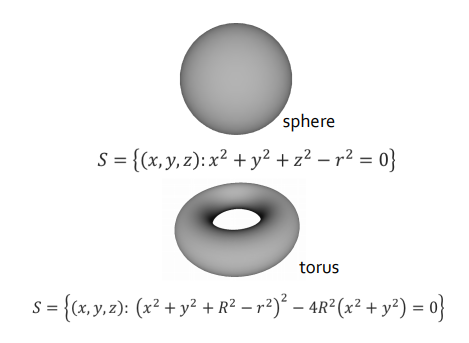
\includegraphics[width=0.5\textwidth]{images/Sfera.png} 
    \caption{Sphere and torus}
    \label{fig:immagine}
\end{figure}
Parametri Surface
\\
Rappresentare un oggetto analiticamente? Ok, ma cosa succede con gli oggetti del mondo reale? Gli oggetti del mondo reale sono difficili da definire in modo analitico.
Cosa succede agli oggetti del mondo reale?
Esistono molte rappresentazioni discrete alternative, a seconda di: tradizione, origine dei dati, comodità per il compito e spazio di archiviazione (dimensioni).
\textbf{Idea}: forme complesse possono essere rappresentate come collezioni di elementi di base. Prendi una serie di elementi semplici e uniscili insieme (in modo strutturato).
\begin{figure}[H]
    \centering
    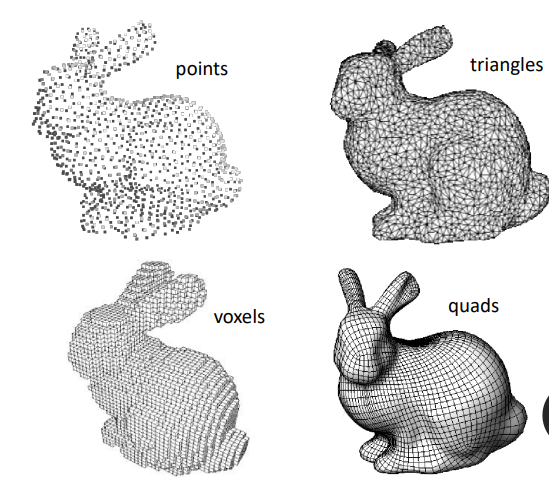
\includegraphics[width=0.5\textwidth]{images/structRep.png} 
    \caption{Rappresentazioni in modo strutturato}
    \label{fig:immagine}
\end{figure}
\subsubsection{Voxels}
Considera le superfici come il confine degli oggetti volumetrici solidi. Definisci una funzione indicatrice che mappa il dominio tridimensionale in un dominio binario discreto (1 significa solido e 0 significa vuoto). Memorizza la funzione in una griglia regolare di voxel.
Anche La \textbf{Signed Distance Field} (SDF) viene  memorizzato in una griglia di voxel. Offre più informazioni rispetto a una semplice mappa di occupazione. Maggior spazio di archiviazione
\begin{itemize}
    \item Pro: Struttura regolare
    \item Contro: Potenzialmente storage massivi
\end{itemize}
Le griglie di voxel possono memorizzare: funzioni indicatrici, campi di distanza (segnati), campi generici (ad esempio, densità, vettori). Maggiore è la risoluzione, maggiore è la dimensione.
\begin{figure}[H]
    \centering
    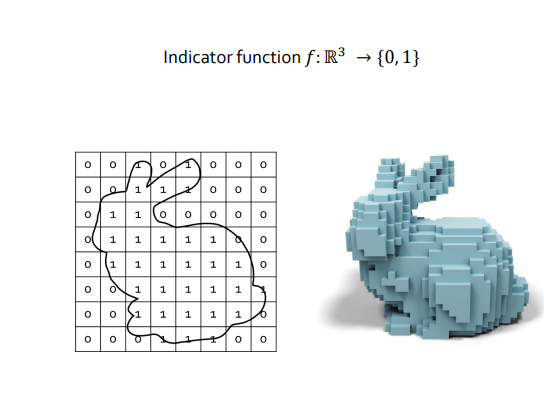
\includegraphics[width=0.5\textwidth]{images/voxels.png} 
    \caption{Rappresentazioni con voxels}
    \label{fig:immagine}
\end{figure}
\subsubsection{Point Clouds}
Collezione non ordinata di sample di punti, 
\begin{itemize}
    \item \textbf{l'origine dei dati}: 3d scans,Lidar, Structure-from-Motion
    \item \textbf{Tasks}: Renderig veloce di dataset di grandi dimensioni, processi iterativi e storage di raw data.
\end{itemize}
Uno dei pro è che i punti sono compatti e facili da gestire e tra i vari contro abbiamo che i punti 
sono irregolari, inconsistenti, non rappresentano davvero superfici.

\begin{figure}[H]
    \centering
    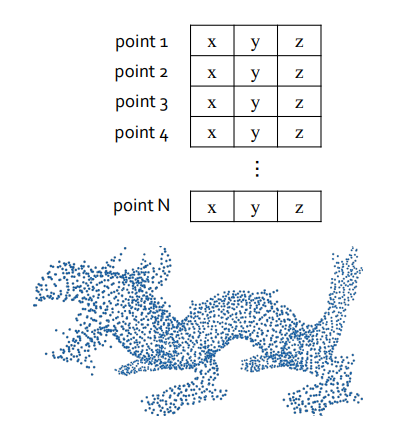
\includegraphics[width=0.5\textwidth]{images/point_Clouds.png} 
    \caption{Rappresentazioni con voxels}
    \label{fig:immagine}
\end{figure}
\subsubsection{Polygonal meshes}
I poligoni sono \textit{building blocks}.
\begin{figure}[H]
    \centering
    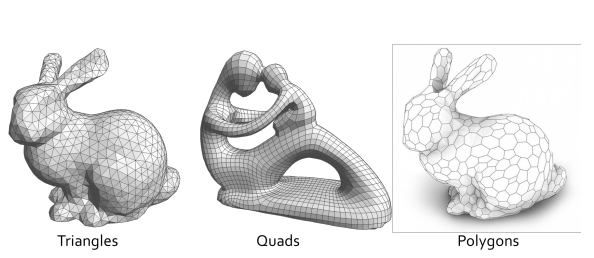
\includegraphics[width=0.5\textwidth]{images/PolygonalMesh.png} 
    \caption{Rappresentazioni con i Poligoni}
    \label{fig:immagine}
\end{figure}
I triangoli come building blocks: Una primitiva molto concisa, con molti vantaggi (pianarità e convessità, potenza di approssimazione...). Rappresentazione di superfici de facto standard per il trattamento della geometria classica.
\begin{itemize}
    \item \textbf{Origine}: modelli CAD, artisti 3D, dati di scansione 3D elaborati, ecc.
    \item \textbf{Compiti}: Rendering 3D (film, videogiochi), applicazioni interattive (GPU), modellazione 3D, elaborazione delle superfici 3D, ...
    \item \textbf{Pro}: Rappresentazione adeguata delle superfici 3D, discretizzazione adattiva, modo più efficiente di memorizzare superfici 3D generiche.
\end{itemize}
Ma comunque quesot metodo è ancora  Irregolare, non ordinato, inconsistente, non orientato.


\begin{figure}[H]
    \centering
    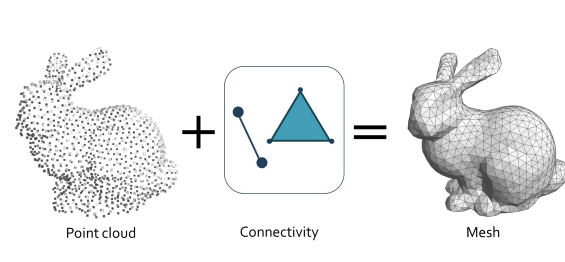
\includegraphics[width=0.5\textwidth]{images/TraingleMeshes.png} 
    \caption{Traingel Meshes}
    \label{fig:immagine}
\end{figure}
\begin{figure}[H]
    \centering
    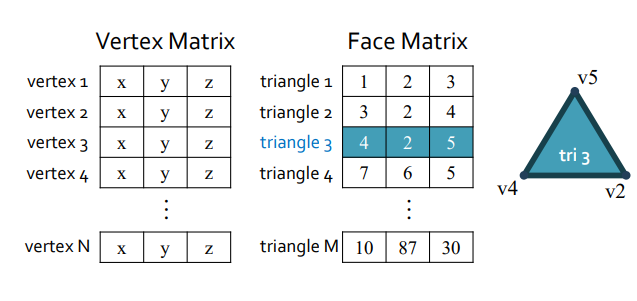
\includegraphics[width=0.5\textwidth]{images/Matricies.png} 
    \caption{Vertex Matrix and Face Matrix}
    \label{fig:immagine}
\end{figure}
\subsubsection{Simplicies}
Gli elementi fondamentali sono chiamati \textbf{Simplicies}.
Un $k$-simplex $\Delta_k$ in $\mathbb{R}^n$, $0 \leq k \leq n$, è l'involucro convesso di $k+1$ punti affinemente indipendenti $A_0, A_1, \dots, A_k$ chiamati vertici.
In $\mathbb{R}^3$ ci sono 4 possibili \textbf{Simplicies}: Punto (0-simplex); Segmento di retta (1-simplex); Triangolo (2-simplex); Tetraedro (3-simplex).
Un simplesso può essere orientato assegnando un ordine ai suoi vertici. Due orientamenti che differiscono per una permutazione pari determinano una stessa orientazione (negativa o positiva).
\begin{figure}[H]
    \centering
    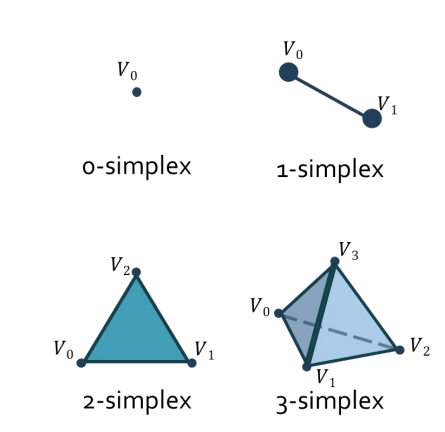
\includegraphics[width=0.5\textwidth]{images/Simplex.png} 
    \caption{Vari tipi di Simplicies}
    \label{fig:immagine}
\end{figure}
\subsubsection{Simplicies complexes}
Una faccia (corretta) di un $k$-simplex $\Delta_k$ è un simplex il cui insieme di vertici è un sottoinsieme non vuoto dell'insieme di vertici di $\Delta_k$. Ad esempio, per un 1-simplex/segmento: i suoi vertici/estremi; 
per un 2-simplex/triangolo: sia i suoi spigoli/segmenti che i vertici.
Un complesso simpliciale finito $\mathcal{K}$ è una collezione finita di simplessi che si incontrano solo lungo una faccia comune, oltre ai loro facce di qualsiasi dimensione.
\begin{figure}[H]
    \centering
    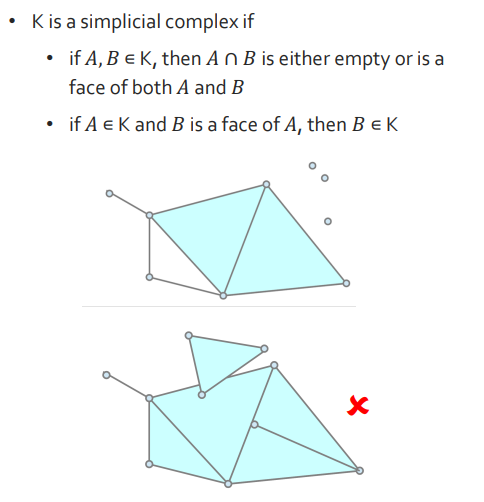
\includegraphics[width=0.5\textwidth]{images/SimpComp.png} 
    \caption{Simplicial Complex}
    \label{fig:immagine}
\end{figure}
La dimensione del complesso simpliciale è la massima dimensione dei suoi simplessi. Un complesso simpliciale $k$-dimensionale è omogeneo se è composto da $k$-simplessi e dalle loro facce (per $k = 2$: è composto da triangoli e tutte le loro facce - senza parti staccate...).
Una rete di bordi è un complesso simpliciale omogeneo unidimensionale.
Una rete di triangoli è un complesso simpliciale omogeneo bidimensionale.
Le reti di triangoli sono complessi simpliciali omogenei bidimensionali.
\begin{figure}[H]
    \centering
    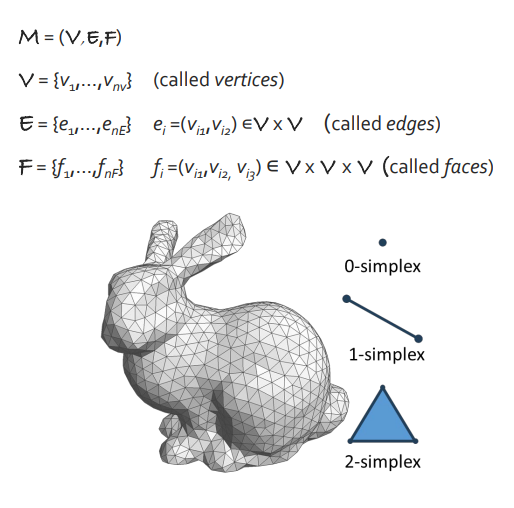
\includegraphics[width=0.5\textwidth]{images/trMesh.png} 
    \caption{Triangle Meshes}
    \label{fig:immagine}
\end{figure}
Sulle reti di triangoli, di solito si distinguono gli \textit{aspetti geometrici} (dove sono posizionati i punti nello spazio) dagli aspetti combinatori (come sono connessi gli elementi).
\begin{itemize}
    \item Due $k$-simplessi $A$ e $B$ sono $m$-adiacenti ($m<k$) se esiste un $m$-simplex che è una faccia corretta sia di $A$ che di $B$
    \begin{itemize}
        \item Due triangoli che condividono un lato sono 1-adiacenti
        \item Due triangoli che condividono un vertice sono 0-adiacenti
        \item Due lati che condividono un vertice sono 0-adiacenti
    \end{itemize}
    \item Due simplessi sono incidenti se uno è una faccia corretta dell'altro
    \begin{itemize}
        \item Due vertici sono adiacenti se sono incidenti su un lato comune
    \end{itemize}
\end{itemize}
\subsection{Star and Link}
\begin{itemize}
    \item \textbf{La stella} di un simplesso $\Delta$ è l'unione di tutti i simplessi che contengono $\Delta$.
    \item \textbf{Il link} di $\Delta$ consiste in tutte le facce dei simplessi nella stella di $\Delta$ che non intersecano $\Delta$.
\end{itemize}
Per una rete di triangoli, il bordo è l'unione di spigoli incidenti a un solo triangolo.
\subsubsection{Surface in Computer Graphics}
Spesso si assume che siano «varietà continue orientabili bidimensionali immerse in $\mathbb{R}^3$».
Intuizione: la superficie di confine di un solido fisico, non degenerato («non degenere» qui significa senza parti infinitamente sottili).
Su una superficie \textit{manifold}, i punti hanno vicinanze topologicamente equivalenti (omeomorfe) o a un disco o a un semidisco (se la superficie ha dei confini).
Le varietà di dimensione 2 e 3 sono modelli matematici convenienti per la rappresentazione degli oggetti tridimensionali.
\begin{itemize}
    \item Validità dei modelli digitali (ad esempio, in medicina, per simulazioni, ecc.)
    \item Strutture dati convenienti (altro da aggiungere nelle prossime lezioni)
\end{itemize}
\subsubsection{From continuos to discrete setting}
La "manifoldness" si riferisce alla caratteristica principale delle varietà di essere spazi che possono essere descritti, almeno localmente, come spazi euclidei.
Per definire la "manifoldness" per le reti di triangoli, abbiamo bisogno di concetti discreti equivalenti di "vicinato" e "disco" (ricordiamo i concetti di stella e link).
(Ricordiamo la definizione nel caso continuo: una superficie è una varietà se ogni punto ha un vicinato che può essere deformato continuamente o in un disco o in un semidisco.)
\begin{figure}[H]
    \centering
    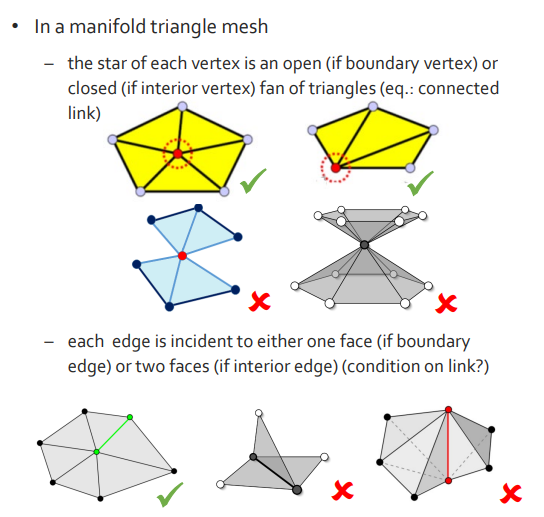
\includegraphics[width=0.5\textwidth]{images/MainfoldTriangle.png} 
    \caption{Triangle Meshes}
    \label{fig:immagine}
\end{figure}
Una varietà combinatoria di dimensione 2 è un complesso omogeneo nel quale ogni vertice è regolare. Si verifica inoltre che tutti i lati siano regolari

\subsection{Orientabilità}
\subsubsection{Tangent and normal vectorscon curves}
Una curva piana parametrizzata e liscia può essere rappresentata come una mappa differenziabile da un intervallo nello spazio dei numeri reali allo spazio euclideo bidimensionale. Il vettore tangente (detto anche vettore velocità) alla curva in un punto è la prima derivata della mappa. Esso fornisce la direzione e la velocità del movimento lungo la curva.
Il vettore normale viene ottenuto ruotando il vettore tangente di 90 gradi. Esso fornisce la variazione (direzione e magnitudine) nella direzione tangente mentre ci muoviamo lungo la curva.
Il \textbf{piano tangente} alla superficie in un punto \( p \) è generato dai vettori tangenti alle curve che passano attraverso \( p \). Il \textbf{vettore normale unitario alla superficie} in \( p \) è il vettore ortogonale al piano tangente in \( p \).
Una superficie è \textbf{orientabile} se è possibile orientare in modo coerente i normali in ogni punto (ovvero, è a due facce). In caso contrario, è non orientabile (ovvero, è a una faccia). Esempi ben noti di superfici non orientabili sono il nastro di Möbius e la bottiglia di Klein.
\subsubsection{Normals on triangle meshes}
Molte operazioni richiedono vettori normali (ad esempio, lo shading). Idea: calcolare i normali ai vertici come media pesata dei vettori normali dei triangoli nella stella (nota: i triangoli sono piani, quindi i normali sono costanti e possono essere calcolati come il prodotto vettoriale di due lati).

Pesi costanti possono dare risultati controintuitivi su reti irregolari. Il ponderamento, ad esempio, in base all'area dei triangoli o agli angoli, può essere di aiuto.
\subsection{Curvature}
La \textbf{curvatura} è una misura che esprime quanto una superficie o una curva si discosta da essere piatta o dritta.
La grandezza del vettore normale è chiamata curvatura. Misura quanto la curva si piega, cioè quanto fortemente la curva si discosta da una linea retta. La curvatura sarà zero per una linea retta.
Su una curva planare, la \textbf{curvatura} è definita come l'inverso del raggio del cerchio osculatore (il cerchio che approssima al meglio localmente la curva, tangente alla curva; linea retta: cerchio di raggio infinito, di conseguenza...).
\subsubsection{Normal curvature on surfaces}
Per estendere la nozione di curvatura dalle curve alle superfici, definiamo la curvatura normale in $p$ come la curvatura della curva planare creata dall'intersezione della superficie in $p$ con il piano generato dal vettore tangente $t$ e il vettore normale $n$ della superficie.
\begin{figure}[H]
    \centering
    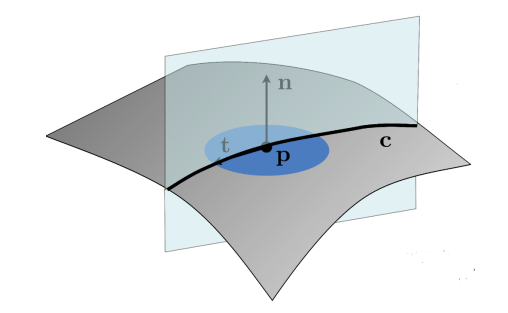
\includegraphics[width=0.5\textwidth]{images/CurvSurf.png} 
    \caption{Curvature Surface}
    \label{fig:immagine}
\end{figure}
La curvatura normale è segnata: è considerata positiva se la curva gira nella stessa direzione del vettore normale della superficie, altrimenti è considerata negativa.
La curvatura normale ha due valori estremali distinti (massimo e minimo), chiamati \textbf{curvature principali}. Questi valori misurano la massima e la minima curvatura della superficie.
Le curvature principali identificano due vettori tangenti unici, chiamati \textbf{vettori principali}, che sono sempre ortogonali l'uno all'altro.
\subsubsection{Mean and Gaussian curvature}
Dalle curvature principali possiamo definire due importanti grandezze: la curvatura media e la curvatura gaussiana.
Intuizione: la curvatura media come operazione logica OR (c'è curvatura almeno lungo una direzione? Ma attenzione a uguale magnitudine e segno opposto) e la curvatura gaussiana come operazione logica AND (c'è curvatura lungo entrambe le direzioni?).
La \textbf{curvatura media} è la media delle curvature principali. Una superficie che ha ovunque curvatura media uguale a zero è una superficie minima (ad esempio, pellicole di sapone).
La \textbf{curvatura gaussiana} è il prodotto delle curvature principali. Il segno della curvatura gaussiana può essere utilizzato per classificare i punti della superficie in tre categorie distinte: ellittiche, iperboliche e paraboliche.
La curvatura gaussiana è spesso utilizzata per l'ispezione visiva al fine di valutare la qualità delle superfici nel design industriale: l'estetica di un oggetto dipende fortemente da come riflette la luce, quindi dalle sue proprietà basate sulla curvatura
\begin{figure}[H]
    \centering
    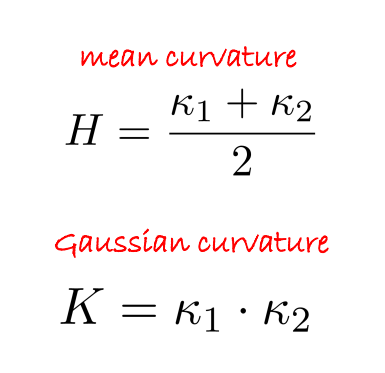
\includegraphics[width=0.5\textwidth]{images/MeanGaussi.png} 
    \caption{Mean and Gaussian curvature}
    \label{fig:immagine}
\end{figure}
\subsection{Geodesics}
Nello spazio euclideo in cui viviamo, la distanza tra due punti è la lunghezza della linea retta che li collega. Le distanze geodetiche generalizzano questa nozione alle superfici: esse misurano i percorsi più brevi tra due punti, se ci si limita a viaggiare sulla superficie stessa.
Le distanze geodetiche sono grandezze intrinseche, poiché non dipendono da come la superficie è inserita nello spazio (possono essere calcolate da creature bidimensionali che vivono sulla superficie senza conoscenza della terza dimensione).
Le distanze geodetiche sono invariate rispetto alle deformazioni della curvatura.
Le mappe che conservano le distanze geodetiche sono chiamate isometrie.
\textbf{Teorema Egregium}:
Afferma che la curvatura gaussiana è una proprietà intrinseca: può essere calcolata da creature bidimensionali che vivono sulla superficie senza conoscenza della terza dimensione.
(Risultato sorprendente! Le curvature principali NON sono intrinseche).
La curvatura gaussiana è invariante sotto isometrie locali.
Una conseguenza del Teorema Egregio è che non esiste alcuna \textbf{isometria} tra una sfera (una superficie di curvatura non nulla) e un piano (una superficie di curvatura nulla). Pertanto, tutte le proiezioni cartografiche distortono la superficie in qualche modo.
\begin{figure}[H]
    \centering
    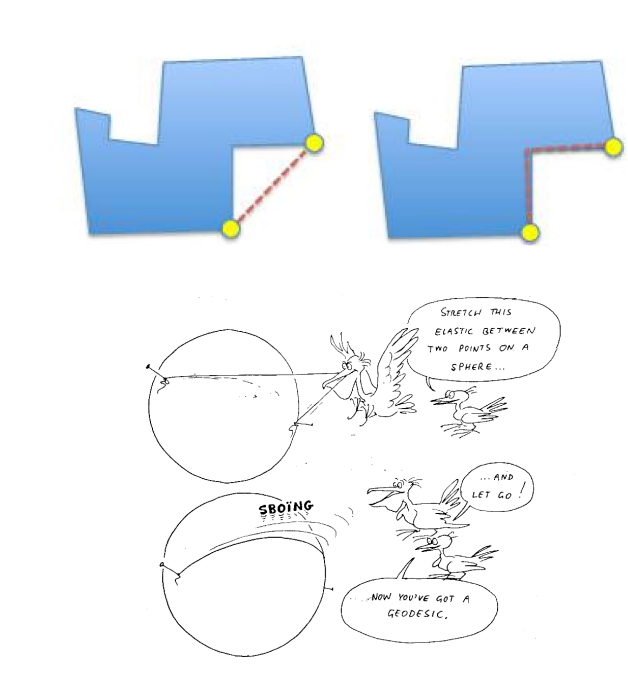
\includegraphics[width=0.5\textwidth]{images/Geode.png} 
    \caption{Geodesics distance}
    \label{fig:immagine}
\end{figure}

\subsection{Genus}
Il \textbf{genere} di una superficie connessa e orientabile è un numero intero che conta il massimo numero di tagli lungo curve semplici chiuse non intersecanti senza disconnettere la superficie. (Abbiamo una definizione più complessa per le superfici non orientabili.)
Il genere è un invariante topologico: se due superfici orientabili hanno lo stesso genere, sono topologicamente equivalenti, il che significa che possono essere deformate continuamente l'una nell'altra (senza strappare né incollare).
\begin{figure}[H]
    \centering
    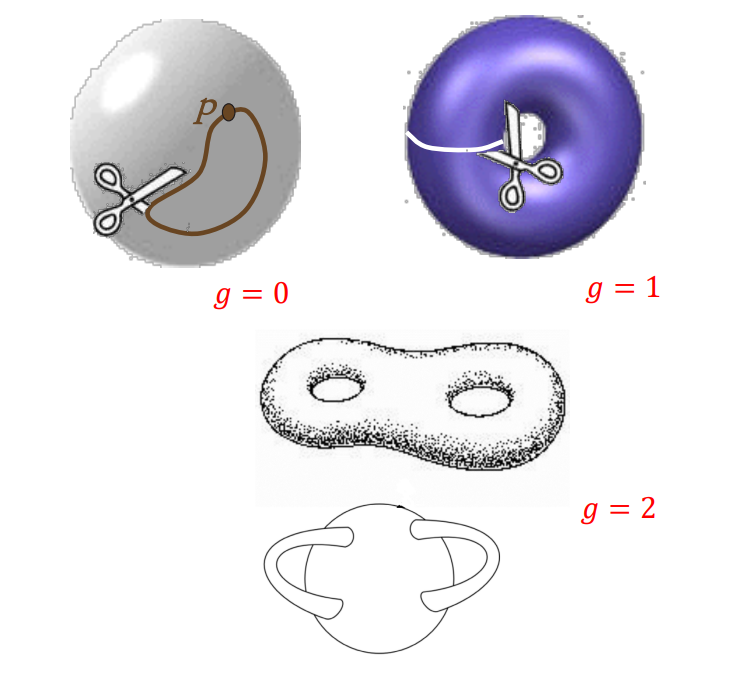
\includegraphics[width=0.5\textwidth]{images/Genus.png} 
    \caption{Genus}
    \label{fig:immagine}
\end{figure}
La caratteristica di Eulero è definita come $\chi = V - E + F$ dove $V$ è il numero di vertici, $E$ è il numero di spigoli, $F$ è il numero di facce.
Si verifica che $\chi = 2 - 2g - b$ dove $g$ è il genere della superficie e $b$ è il numero di bordi.





